\chapter{同時送信フラッディング}

\section{マルチホップネットワークの特徴}
マルチホップとはノードからノードへバケツリレーのようにデータを転送していく方法である.マルチホップネットワークは,ノードが中継することによって直接波では届かない場所までデータを届けることができるという特徴がある.
全てのノードが受信/送信両方を行い,中継を繰り返すことでネットワーク全域にデータを広める.具体的には,送られてきたデータに対して受け取ったノードが,データの目的地に応じて送り出す経路を変える.これをルーチングという.このルーチングをどのように決めるのか・行うのかの決まり事がルーチングプロトコルである.ルーチングプロトコルはさまざまなものが考案されているが,大きく二つにわけられる.

\begin{itemize}
    \item プロアクティブ型 端末間で常に情報をやり取りし,経路表を更新し続ける方法(ex.OLSR)
    \item リアクティブ型 端末からの要求があった時にのみ経路表の更新を行う方法(ex.AODV,ZigBeeもAODVべース)
\end{itemize}
従来のマルチホップ通信は干渉を通信品質を下げるものとして捉え,複雑なルーチングプロトコルによって干渉を避けることに焦点を当てていたが,同時送信フラッディングは送信タイミングの調整によって干渉による影響を復調が可能な範囲内に抑えること,マルチパスにすることで成功確率を上げることに焦点を当てている.
また,同時送信フラッディングは,各ノードが経路情報を持たずにフラッディングのみで転送を行い,ルーチングを考えない.ノードが互いの通信状態について関知しないという点で従来のマルチホップ通信と異なる.
つまり,同時送信フラッディングでは,ルーチングを廃したフラッディングによるデータ転送を行っている同時送信フラッディングでのデータ転送は基本的にマルチパス転送であり,ユニキャスト通信において用いられるバックオフ時間が不要である.このことから,高信頼かつ低遅延な通信を実現可能である.

\section{同時送信フラッディング概要}
同時送信フラッディングは2011年に提唱されたZigBeeにおけるマルチホッププロトコルの一つである.
同時送信フラッディングの主な特徴は,建設的干渉と時刻同期である.ここで,建設的干渉とは,空間や時間,周波数が同一の信号を送出した場合においても,元のデータが復調可能である現象であり,受信ノードにおける各送信ノードからの電波到来時間差が0.5\si{\micro\second}以内に収まる場合に発生すると述べられている\cite{Effi}.その後の研究で建設的干渉が起きる場合もあれば起きない場合もあることがわかり,データの復調の成功が建設的干渉によるものなのかマルチパスによるものなのか厳密に区別した評価は行われていない\cite{revising}.しかし,受信ノードにおける各送信ノードからの電波到来時間差が0.5\si{\micro\second}以内に収まる場合に高い成功率を実現していることは事実である.
また,この0.5\si{\micro\second}は,実験から得られた値である.この値はZigBee\cite{zigbee}の変調方式に関係している.詳しくは\ref{sec:modulation}章で述べる.
また,受信ノードにおける各送信ノードからの電波到来時間差を0.5\si{\micro\second}以内に収めるためには,ノード間の正確な時刻同期が必要である.これはパケットに含まれる中継カウンタと伝送時間の計算から,Initiatorと転送ノードを相対的に時刻同期することで実現している.詳しくは\ref{sec:time}章で述べる.

 また,同時送信フラッディングは,従来の転送手法と比較して信頼性が高く,部分的な通信障害やノードの障害が同時送信フラッディングの転送性能に与える影響がわずかであることが実験によって実証されている.先行研究\cite{lowper}によると,Wi-Fi干渉による通信障害に対して平均99\%以上のデータ収集率を示し,デューティ比も低い値を維持している.ここでいうデューティ比とは,起動時間に占める送信時間の割合のことで,この値が大きいということは再送が多いということを意味する.
 ノード障害においても,既存のプロトコルDozerがデータ収集率を96\%に落としたのに対し,同時送信フラッディングを用いたプロトコルによる通信は常時99\%以上の安定したデータ収集率を示している.

\section{ZigBeeについて}
\label{sec:modulation}
ZigBeeにおける物理層とMAC層は,IEEE802.15.4規格を適用している.IEEE802.15.4規格では拡散方式がDSSS(Direct Sequence Spread Spectrum),変調方式がO-QPSK(Offset-Quaternary Phase Shift Keying)である.ZigBeeのプロトコルスタックを図\ref{fig:stack}に示す.本研究の焦点はホストノードの選び方が同時送信フラッディングに及ぼす影響だが,同時送信フラッディングの原理がZigBeeの変調方式に根差しているため軽く触れておく.

\begin{figure}[H]
  \centering
  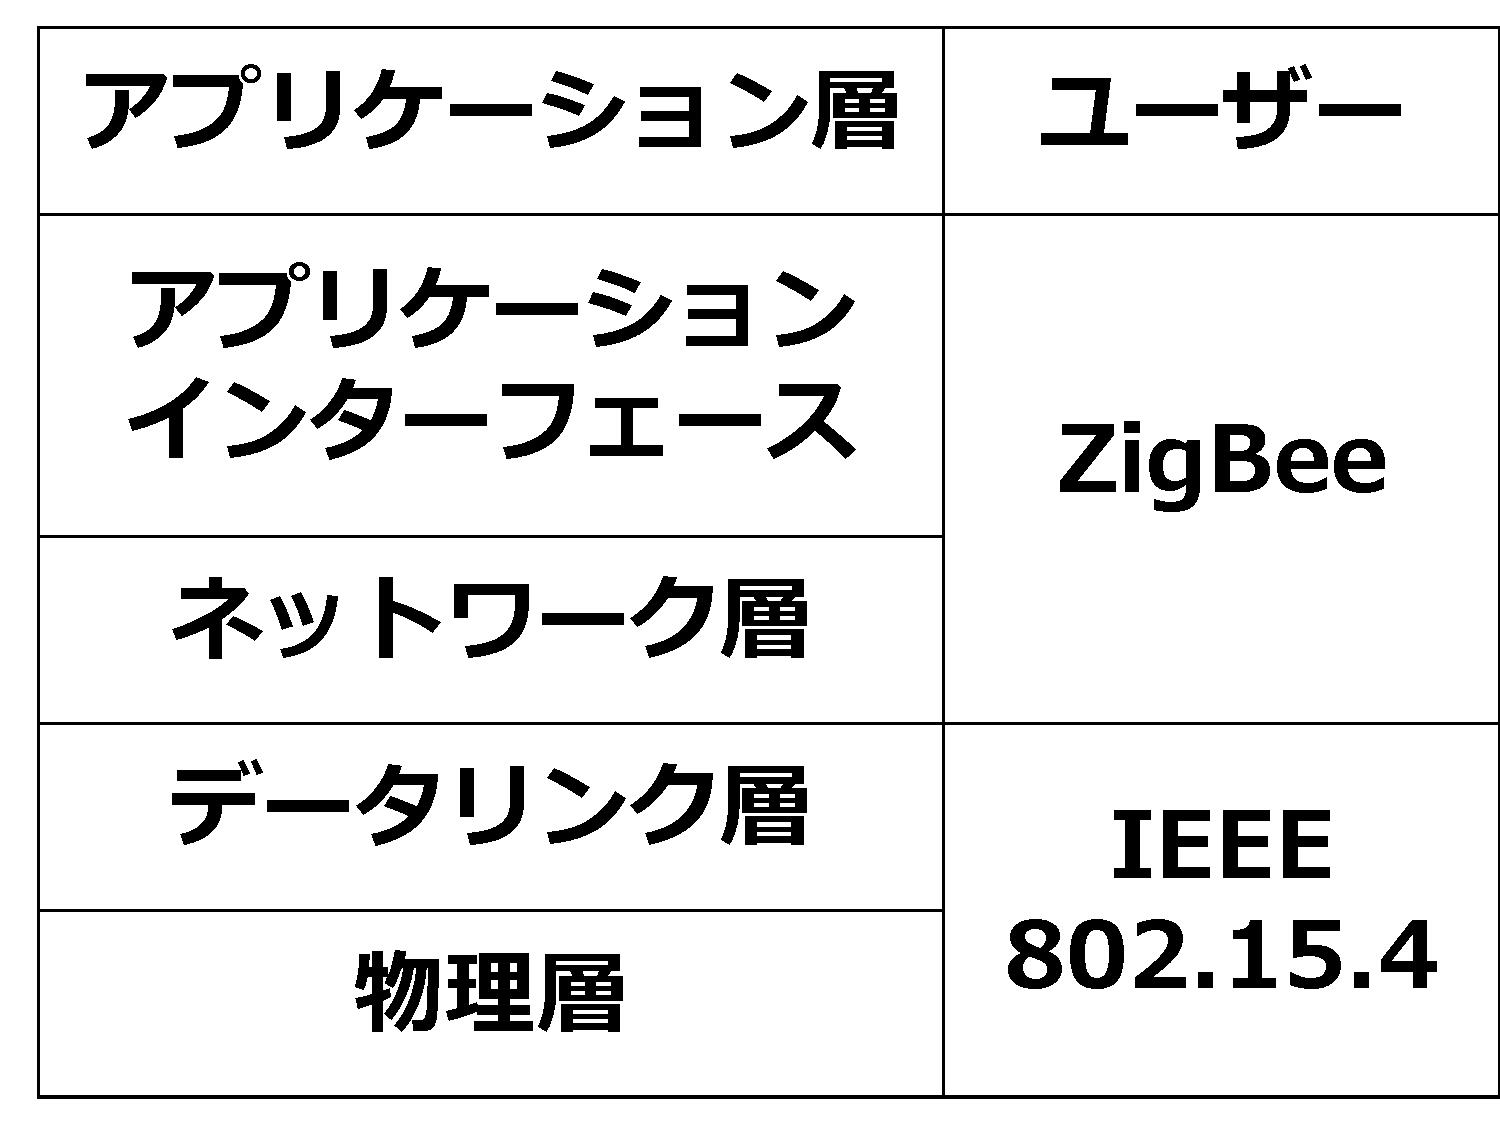
\includegraphics[width=0.3\textwidth]{figures/prostack.pdf}
  \caption{ZigBeeのプロトコルスタック}
  \label{fig:stack}
\end{figure}
%https://www.oki.com/jp/Home/JIS/Books/KENKAI/n200/pdf/200_R19.pdf


DSSSでは信号を4ビットごとに分け,そのかたまりを16パターンのシンボルにマッピングする.これをさらに32ビットの疑似ランダムノイズ(PN)符号(これをチップという)と掛け合わせて広い帯域に拡散させる.すると図\ref{fig:DSSS1}に示すように信号は広帯域に広がり,出力が下がる.復調は逆の手順で行われる.信号を広帯域に拡散させることの利点は,出力が下がることで信号が互いに干渉しづらくなることである.また,突発的なノイズや妨害は図\ref{fig:DSSS2}に示すように復調の過程で拡散され,影響が少なくなるため耐性がある.
O-QPSK(Offset-QPSK)は0と1の二値信号でデータを伝送するデジタル変調方式の一種である.基準信号を位相変調するのがPSKで,4段階で位相の変調を行うのがQPSKである.O-QPSK(Offset-QPSK)は先述のシンボルを,奇数シンボル(Qデータ)と偶数シンボル(Iデータ)間で$\pi$/2に相当する時間分ずらして送信する方法である.信号成分の振幅と位相は極座標において半径と位相で表されるが,これを極座標系から直交(X,Y)座標系に変換したものがQ/Iデータである.
この$\pi$/2差を得るために同位相Qチップは,逆位相Iチップに対してTc=0.5\si{\micro\second}だけ遅延される~\cite{Effi}.

\begin{figure}[H]
  \centering
  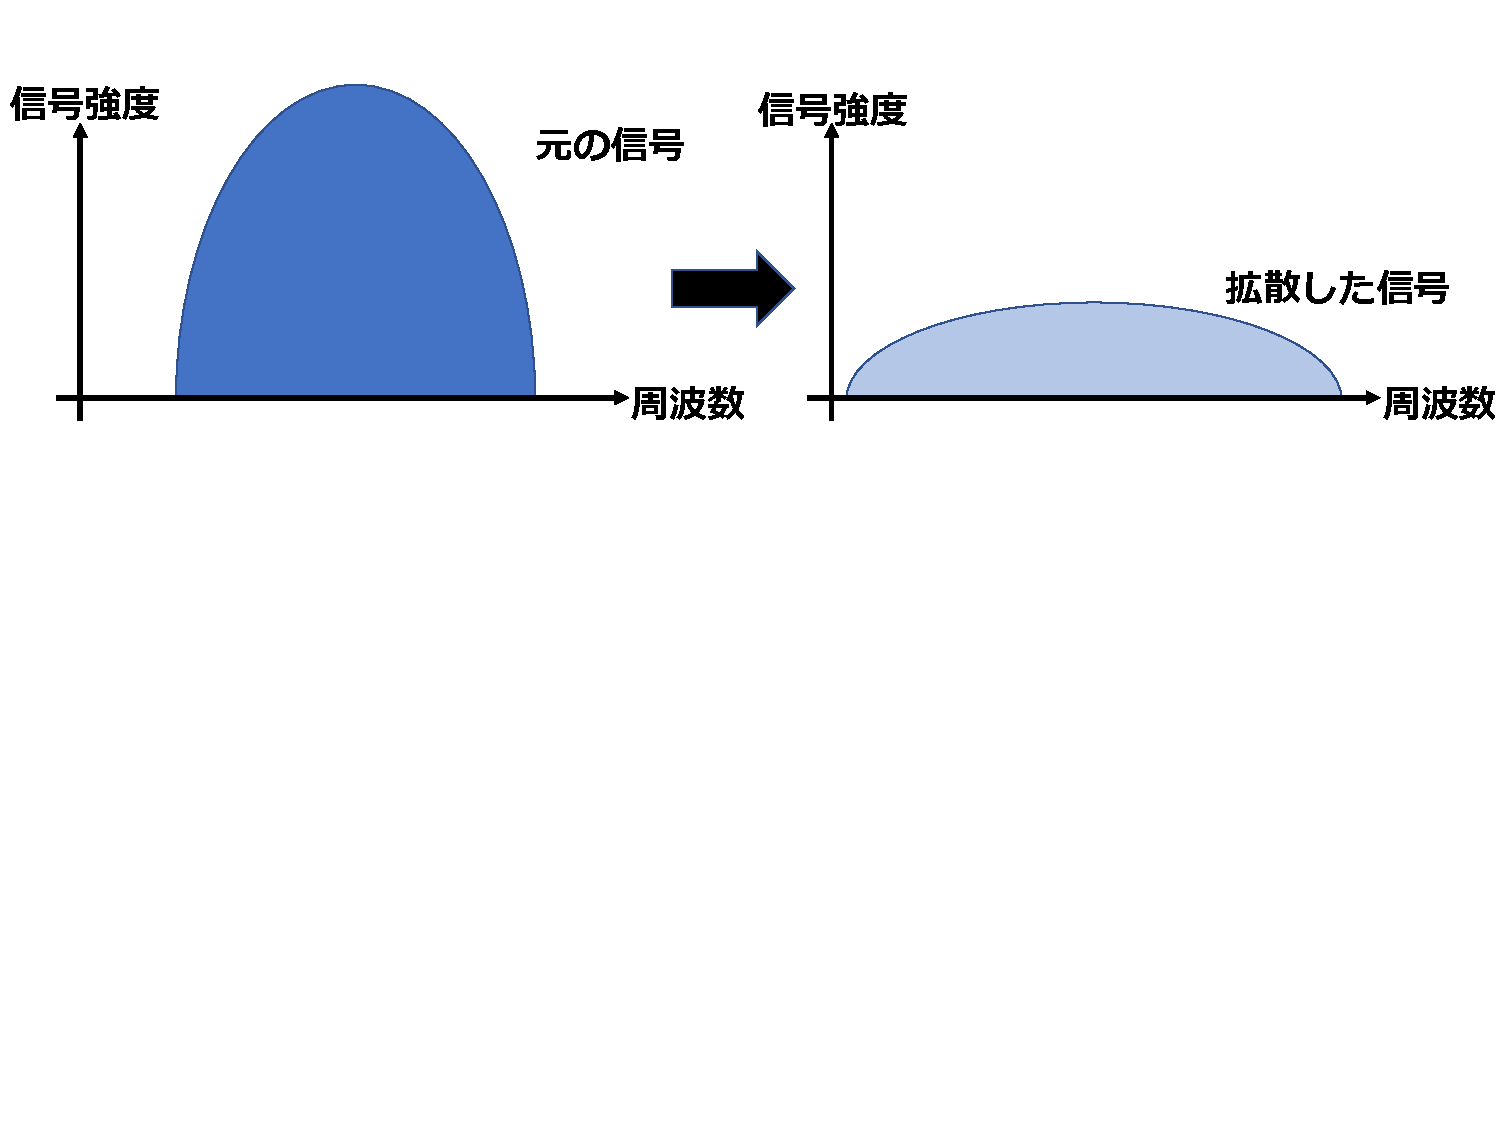
\includegraphics[width=0.8\textwidth]{figures/6.pdf}
    \vspace{-40mm}
  \caption{DSSS拡散によって元信号の周波数帯が広がる様子}
  \label{fig:DSSS1}
\end{figure}

\begin{figure}[H]
  \centering
  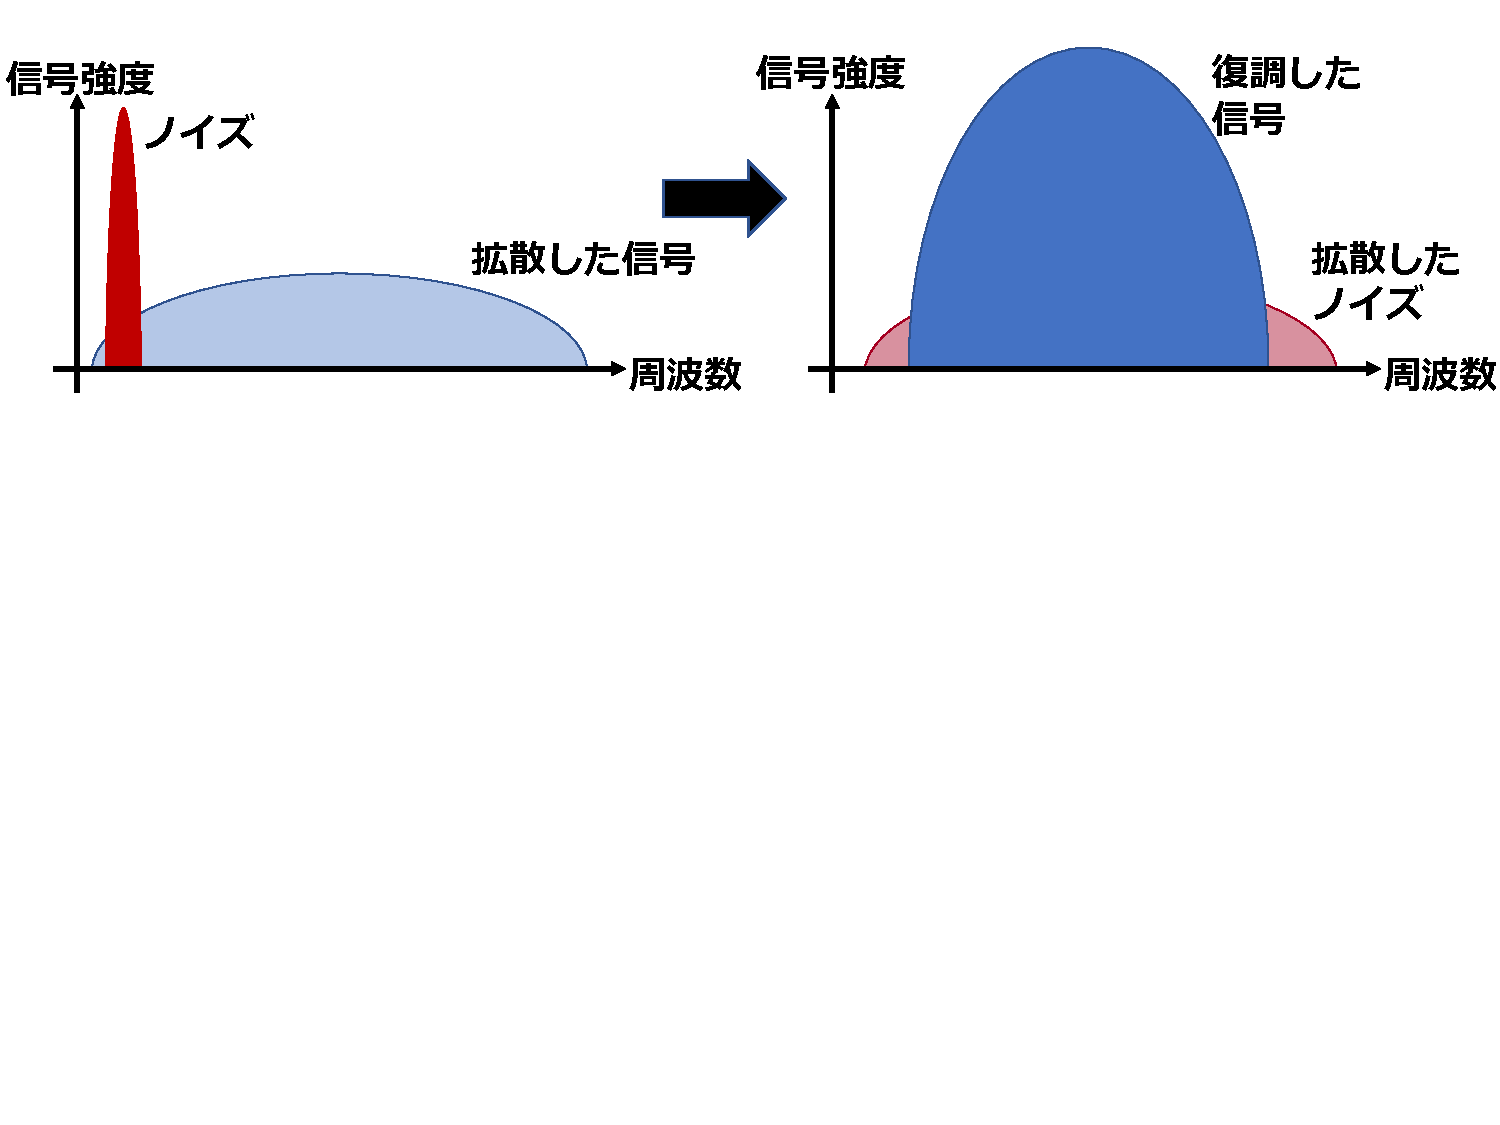
\includegraphics[width=0.8\textwidth]{figures/7.pdf}
  \vspace{-50mm}
  \caption{復調におけるノイズ処理}
  \label{fig:DSSS2}
\end{figure}
%https://ascii.jp/elem/000/000/462/462443/

\section{同時送信フラッディング詳細}
以下の図\ref{fig:ctf_ju}は同時送信フラッディングのフローチャートである.フローチャートにおいてはフローチャート上で隣り合うノード同士が通信可能とする.また,ホストノードやInitiatorとノード1,2,3は同じハードウェアであり,状況に応じて役割を変更している.今回はホスト障害後にnode1が新ホスト,Initiator同じノードが続行するという状況をフローチャートに示した.加えて,中継カウンタ(c=i)が同じ転送は,フローチャート上で,仕様上タイミングがずれて見えるが,実際は同じ時間に送信されていると見なす.また,フローチャート上の赤いライフラインは,ノードが電源をonにして待機している状態,白いライフラインはノードが転送中であることを示している.図\ref{fig:ctf_ov}は同時送信フラッディングを別の形で示したものである.緑色のノードはフローチャートにおいてライフラインがない状態,グレーのノードがフローチャートにおける赤いライフラインを示している.
フローチャートとノード図の対応を表\ref{tab:taio}に示す.

\begin{table}[H]
  \caption{対応表}
  \begin{tabular}{c|c} \hline \hline
     フローチャート& ノード図  \\\hline
     host&ホストノード(赤)\\
    Initiator&上段〇1の黄色ノード,下段〇1の黄色ノード\\
    node1,2,3&上記2つ以外のノード\\\hline
     ライフラインなし & 休眠ノード(緑)\\
     赤いライフライン & 受信待機ノード(灰色)\\
     白いライフライン & 青い円内の灰色ノード\\\hline\hline
  \end{tabular}
  \label{tab:taio}
\end{table}

同時送信フラッディングはスケジューリングフェーズとデータ転送フェーズにわかれる.
図\ref{fig:ctf_ju}においては赤いコメントでスケジューリングフェーズと転送フェーズの区切りを示している.
(1)図\ref{fig:ctf_ov}における最初のスケジューリングフェーズ(図\ref{fig:ctf_ov}だと〇0)\\
ホストノードからその他のノードにスケジュールパケットを送り,時刻同期(詳しくは\ref{sec:time}章で述べる)とノードの生存確認及びノード間の通信確認を行うフェーズである.全ノードとやり取りが済むと転送フェーズに移る.\\

(2)図\ref{fig:ctf_ov}における最初の転送フェーズ(図\ref{fig:ctf_ov}だと上段の〇1-4)\\
Initiatorが最初の送信を行い,Initiatorからの信号の到達範囲(青い円)内のノードがパケットを受信する.パケットを受信したノード(Receiver)は受信後即座に転送を行い転送ノードとしての役割を果たす.また1フェーズにおける転送回数が設定されていて,その上限に達したノードは,転送後電源をoffにする(図\ref{fig:ctf_ov}だと緑の丸の休眠ノード).理論上はホップ数$\times$伝送時間で図\ref{fig:ctf_ov}〇4の状態(ネットワークにデータが行き渡った状態)になる.\\

(3)二回目以降の転送フェーズ(図\ref{fig:ctf_ov}だと下段の〇1-4)\\
スケジューリングフェーズの段階で休眠後最初に目覚めるノード(Initiator)が指定されている.Initiatorが目覚める時間は直前の転送フェーズが終わった直後なので,ホップ数$\times$伝送時間で大体見当がつく.Initiator以外のノードはスケジューリングフェーズでInitiatorに対して相対的に時刻同期が行われているため,そこから逆算してデータが送られてくる直前に電源をonにし,転送後即座にoffにすることができる.転送を行うとき以外は電源をoffにしているため省電力である.

\vspace{-30mm}
\begin{figure}[H]
  \centering
  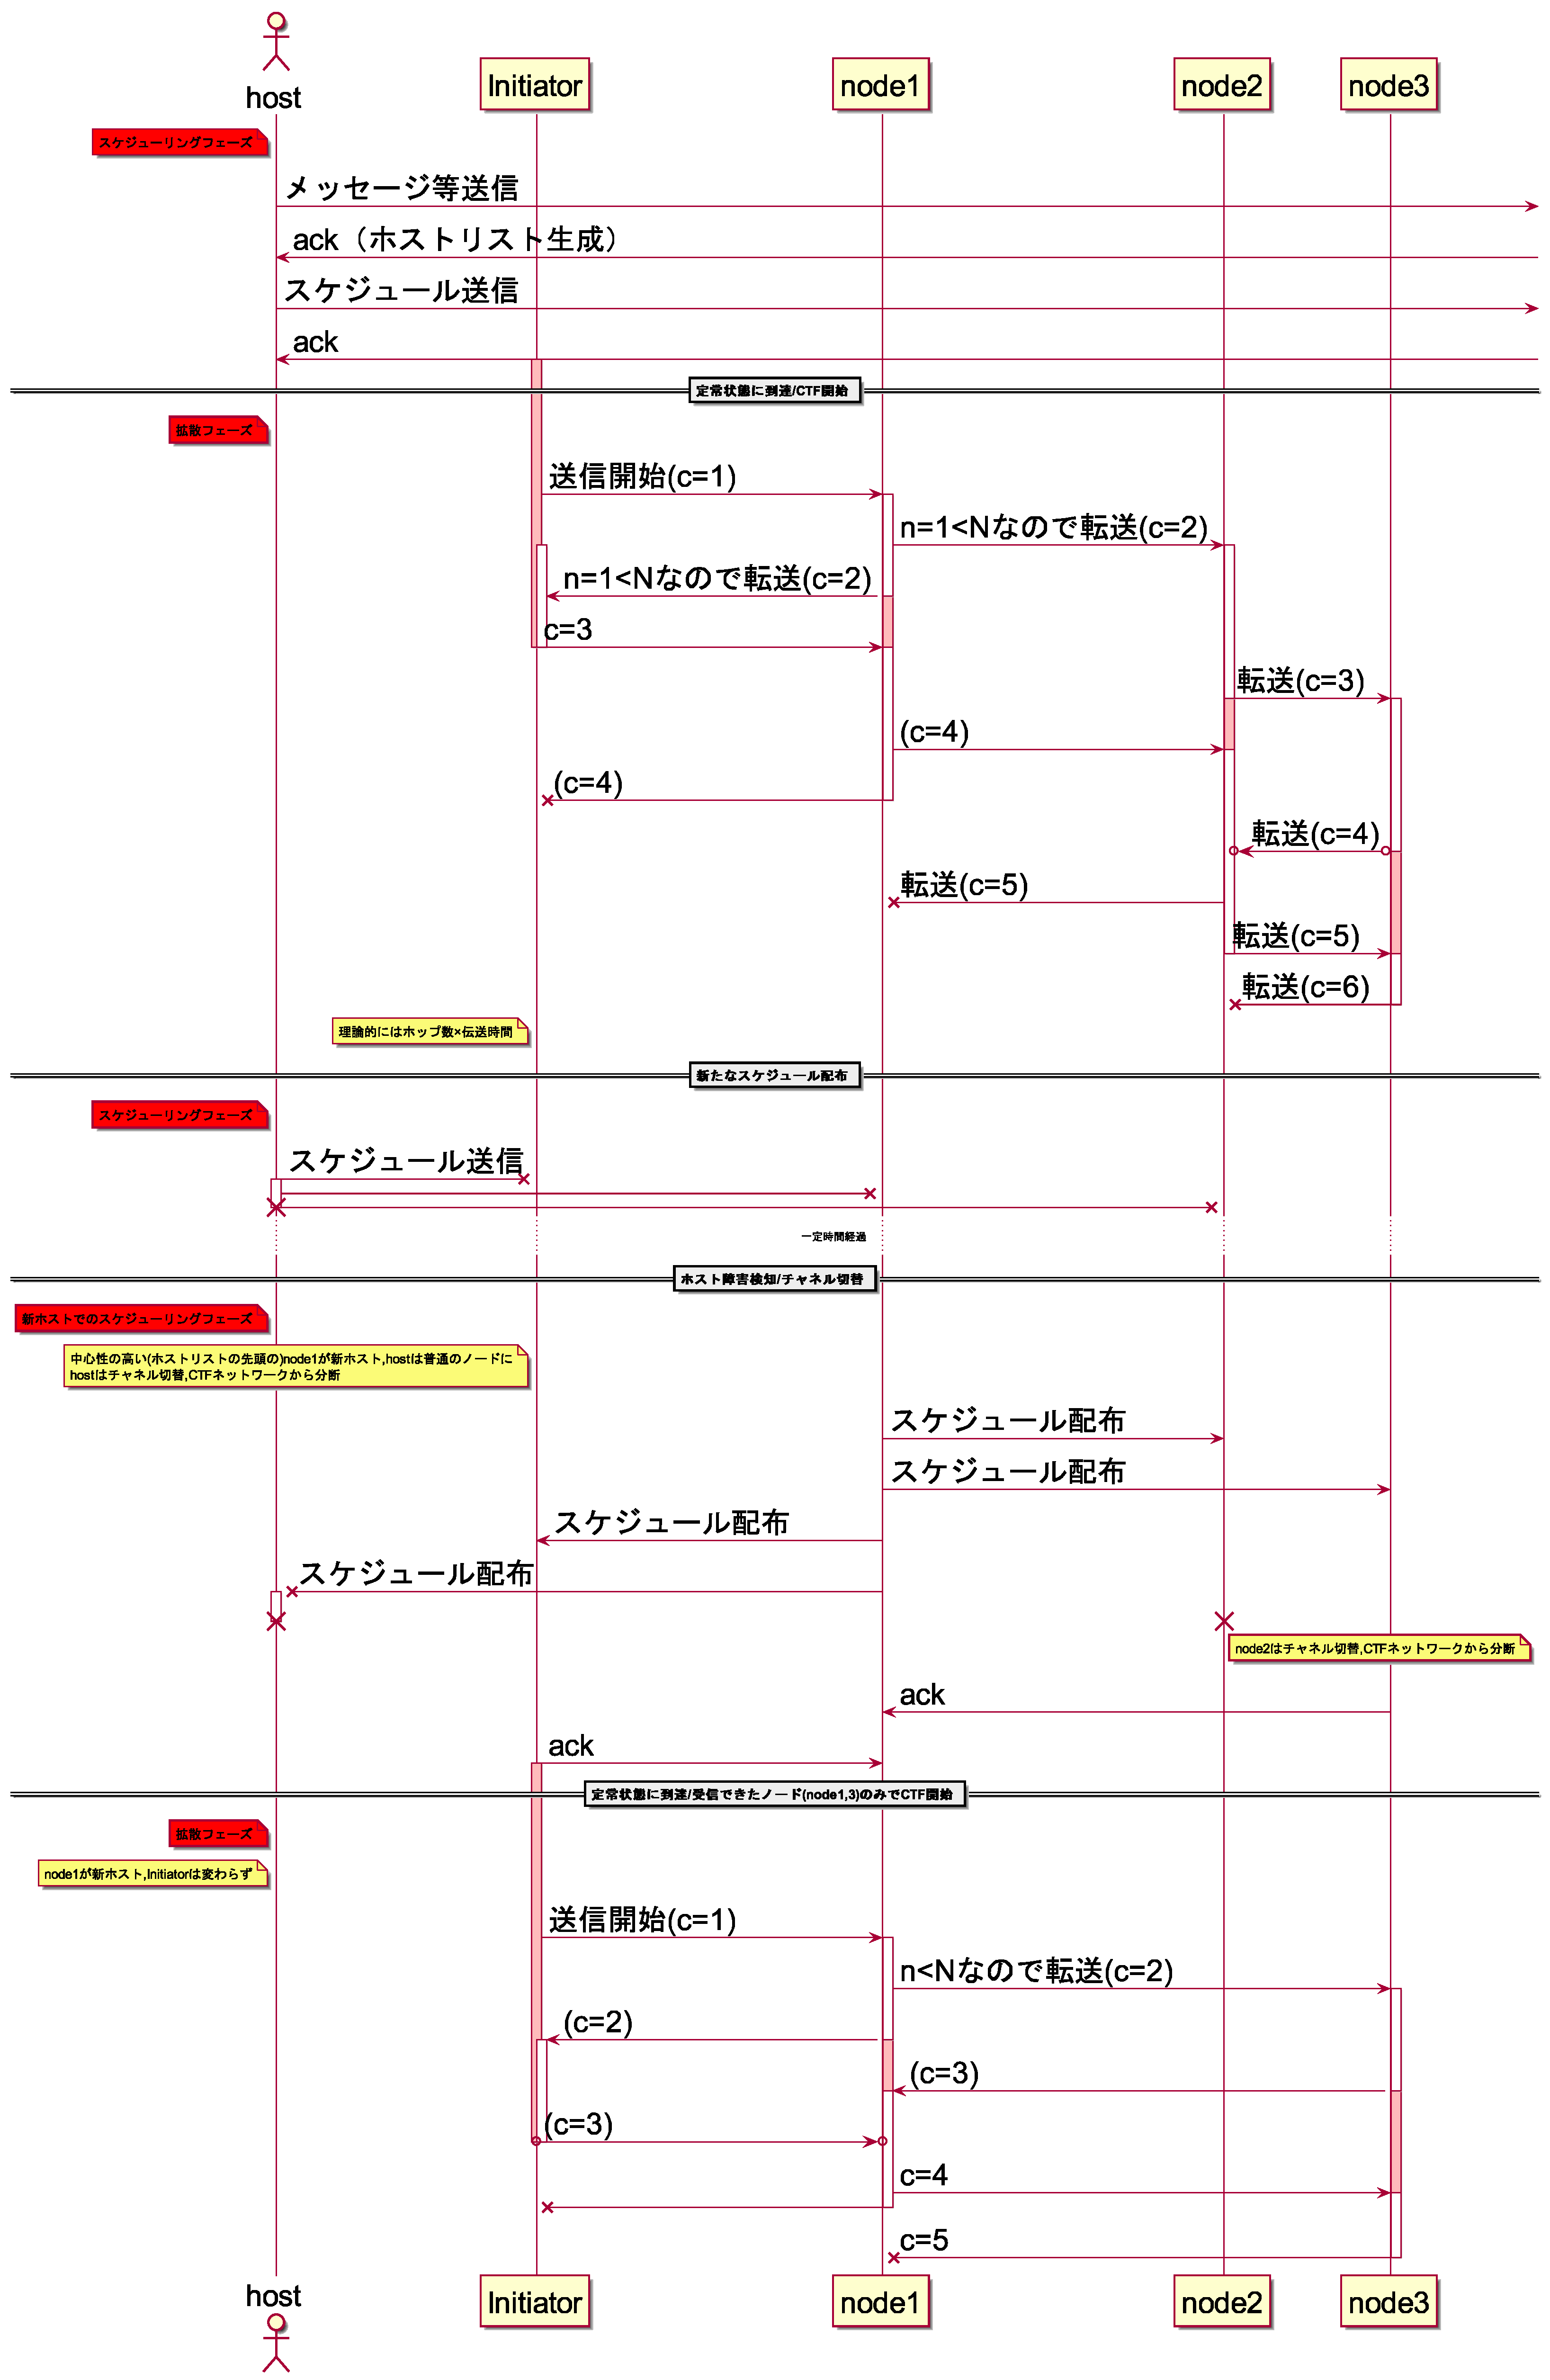
\includegraphics[width=1\textwidth]{figures/sequence_jurai.eps}
  \caption{同時送信フラッディングの従来フローチャート}
  \label{fig:ctf_ju}
\end{figure}

 \begin{figure}[H]
\centering
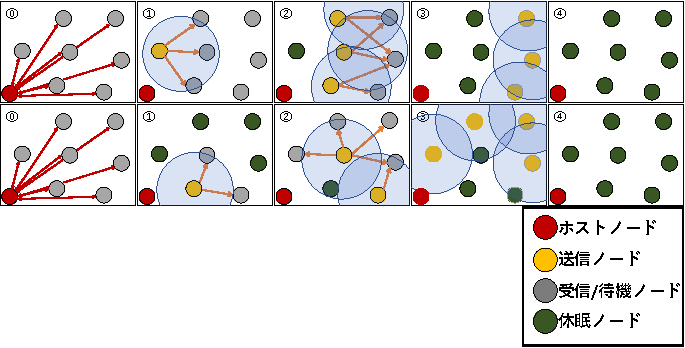
\includegraphics[width=0.85\textwidth]{figures/newctf.pdf}
 \vspace{-1mm}
 \caption{同時送信フラッディング概要}
 \label{fig:ctf_ov}
\end{figure}

同時送信フラッディングの参加ノードは,全てのノードが状況に応じてホスト,Initiator,Receiverの役割を担う~\cite{Effi}.Initiatorは,フラッディング開始時に最初の送信を行うノードである.
Reciverは,データが届いたことを検知した直後,即座に転送するノードである.Receiverのイベントのトリガーは無線信号である.Receiverはデータ受信後即座にデータを転送する.このように状況に応じて各ノードが適した役割を担い,マルチホップでデータをネットワーク内に拡散している.
Receiverのトリガーは無線信号の受信であるが,最初の送信を行うInitiatorはホストノードから受け取ったスケジュールにしたがって指定された時間に送信を開始する.転送フェーズが終了し全てのノードが電源offにしても,Initiatorは指定時間に電源をonにする.Initiator以外のノードはInitiatorに対し,相対的に時刻同期しているため,Initiatorの復帰時間から逆算して自分の復帰時間を知ることができる.詳しくは\ref{sec:time}で述べる.
また,永遠に転送が続くことを回避するため,あらかじめ決められた一定回数の転送を終えたノードは電源を切って待機する.図\ref{fig:ctf_ov}は転送回数を1回,図\ref{fig:ctf_ju}は転送回数を2回としたときである.

\section{ホスト障害時の動作}

通信障害とノード障害が同時送信フラッディングに与える影響が少ないことは先で述べたが,同時送信フラッディングの管理を担うホストノードに障害が起きると時刻同期とスケジューリングができなくなり支障が出る.既存研究~\cite{lowpower}では,全ノードにスケジューラを配置し,状況に応じてスケジューラの無効/有効を切替えることで,ホストノードが正常に動作しなくなった場合に次のホストノードを選出し,障害に対応している.また,同一チャネル上に複数ホストノードが同時に存在することを回避するため,あらかじめ各ノードがチャネルと一対一対応のホストリストを保持している.

次に同時送信フラッディングのホスト障害時の動作について述べる.図\ref{fig:ctf_ju}においては,赤いノートの二つ目のスケジューリングフェーズと新ホストでのスケジューリングフェーズと最後の拡散フェーズがホスト障害時の動作に該当する.
 
 \begin{itemize}
    \item 待ち時間内にホストノードからのスケジュールパケットが到着しないことで障害検知(図\ref{fig:ctf_ju}:二つ目のスケジューリングフェーズ,図\ref{fig:host1})
    \item リストを参照し,次のチャネルに切替える(図\ref{fig:host2})
    \item チャネルと一対一対応のホストノードが自分かどうか判断
    \item 自分が指定されたノードならホストノードに,でなければ待機(図\ref{fig:host3})
    \item 新ホストがスケジュールパケットを配布(図\ref{fig:ctf_ju},新ホストでのスケジューリングフェーズ)
    \item 新ホストに指定されたInitiatorが最初の送信を行い拡散フェーズ開始(図\ref{fig:ctf_ju},最後の拡散フェーズ)
\end{itemize}

 \begin{figure}[H]
\centering
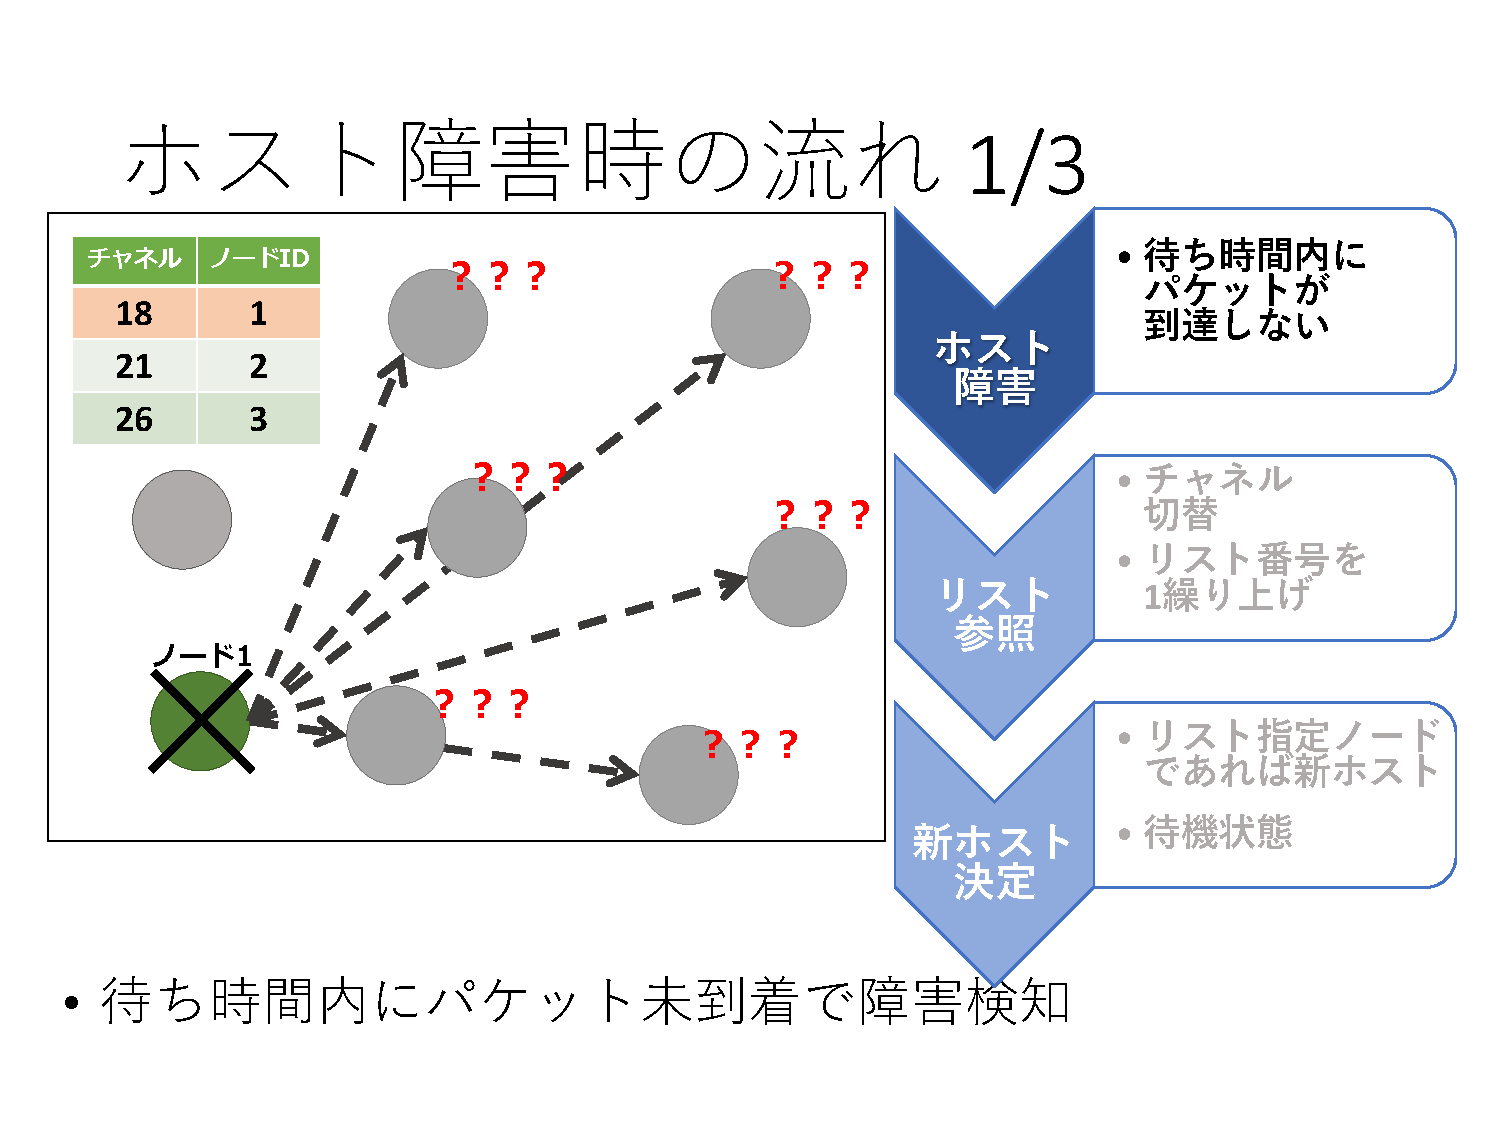
\includegraphics[width=0.8\textwidth]{figures/host1.pdf}
 \caption{ホスト障害1}
 \label{fig:host1}
\end{figure}

 \begin{figure}[H]
\centering
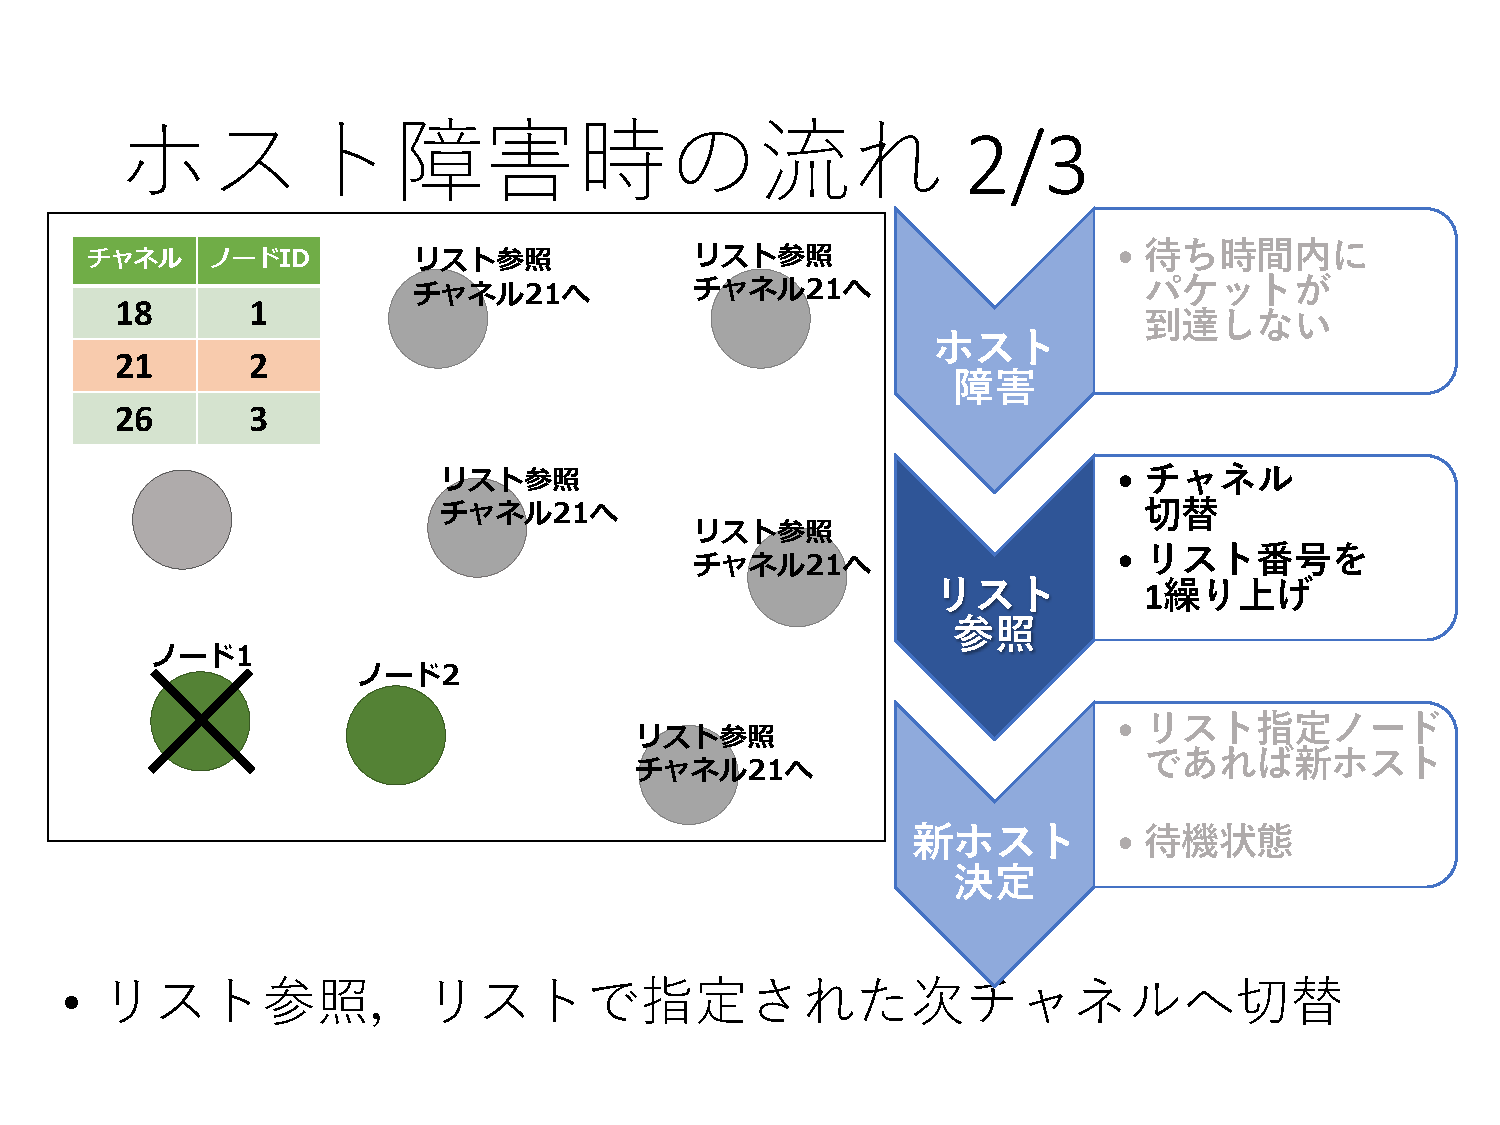
\includegraphics[width=0.8\textwidth]{figures/host2.pdf}
 \caption{ホスト障害2}
 \label{fig:host2}
\end{figure}

 \begin{figure}[H]
\centering
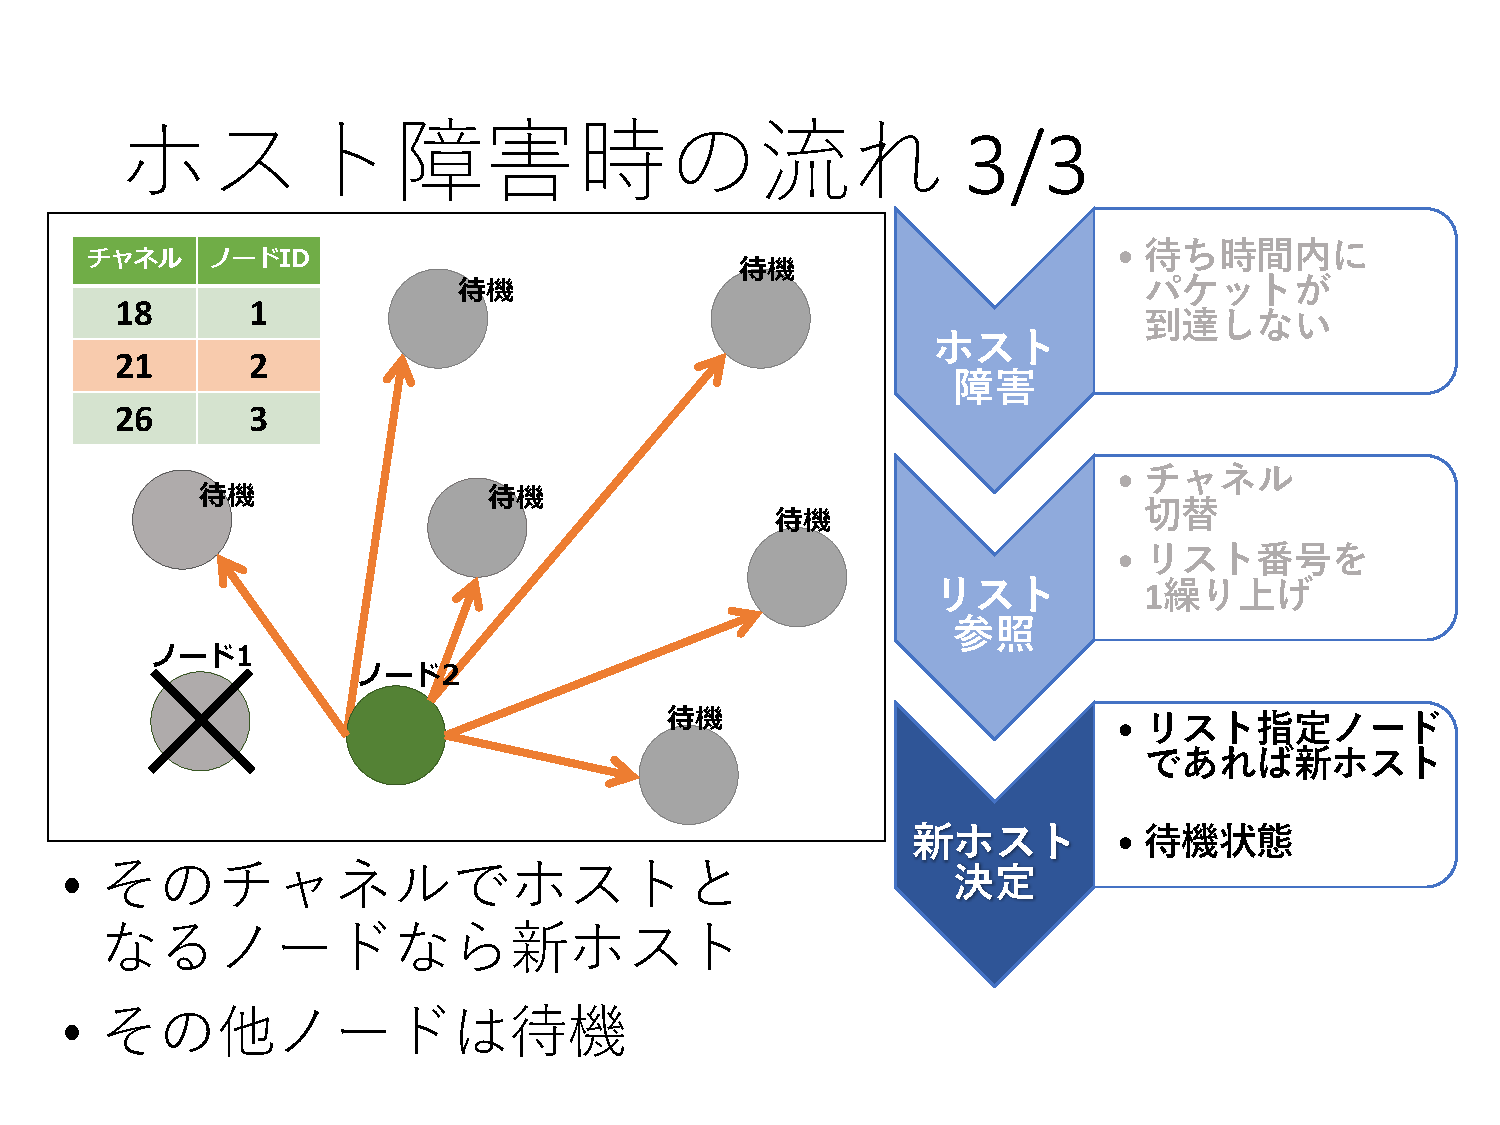
\includegraphics[width=0.8\textwidth]{figures/host3.pdf}
 \caption{ホスト障害3}
 \label{fig:host3}
\end{figure}

図\ref{fig:host1}に示すように,各ノードが一定時間$T_{hf}$内に現在のホストノードからパケットを受信せず,障害発生を認識すると,リストを参照し次のチャネルに切替える.
このとき,自ノードがリストで指定されている場合,ホストノードとして動作する.チャネル切替後に一定時間経過しても新ホストからのパケットを受信できない場合,再度チャネルを切替える.このように,各ノードがホストノードの通信の有無によりホストノードの生存確認を行うことで,通信環境に応じたホスト選択を可能にしている.一方,この従来手法では,何らかの要因で待ち時間$T_{hf}$以内に新ホストノードからの通信を受信できないことが繰り返された場合,ノードがチャネルを切替え続け,正常に新ホストからの通信を受信したノードと合流できず,ネットワークが分断される可能性がある.



 \section{同時送信フラッディング時刻同期}
 \label{sec:time}
次にノード間の時刻同期について述べる.まず,パケットには中継カウンタcが含まれている.ノードはカウンタを1増やしてからパケットを転送する.そのためノードは中継カウンタの値からそのパケットが何回転送されたものか判別できる.また,ノードはデータ受信時にタイムスタンプを記録しており,カウンタcとc+1のパケットの送信開始時間差$T_{slot}$を推定することができる(図\ref{fig:time}).

\begin{figure}[H]
\centering
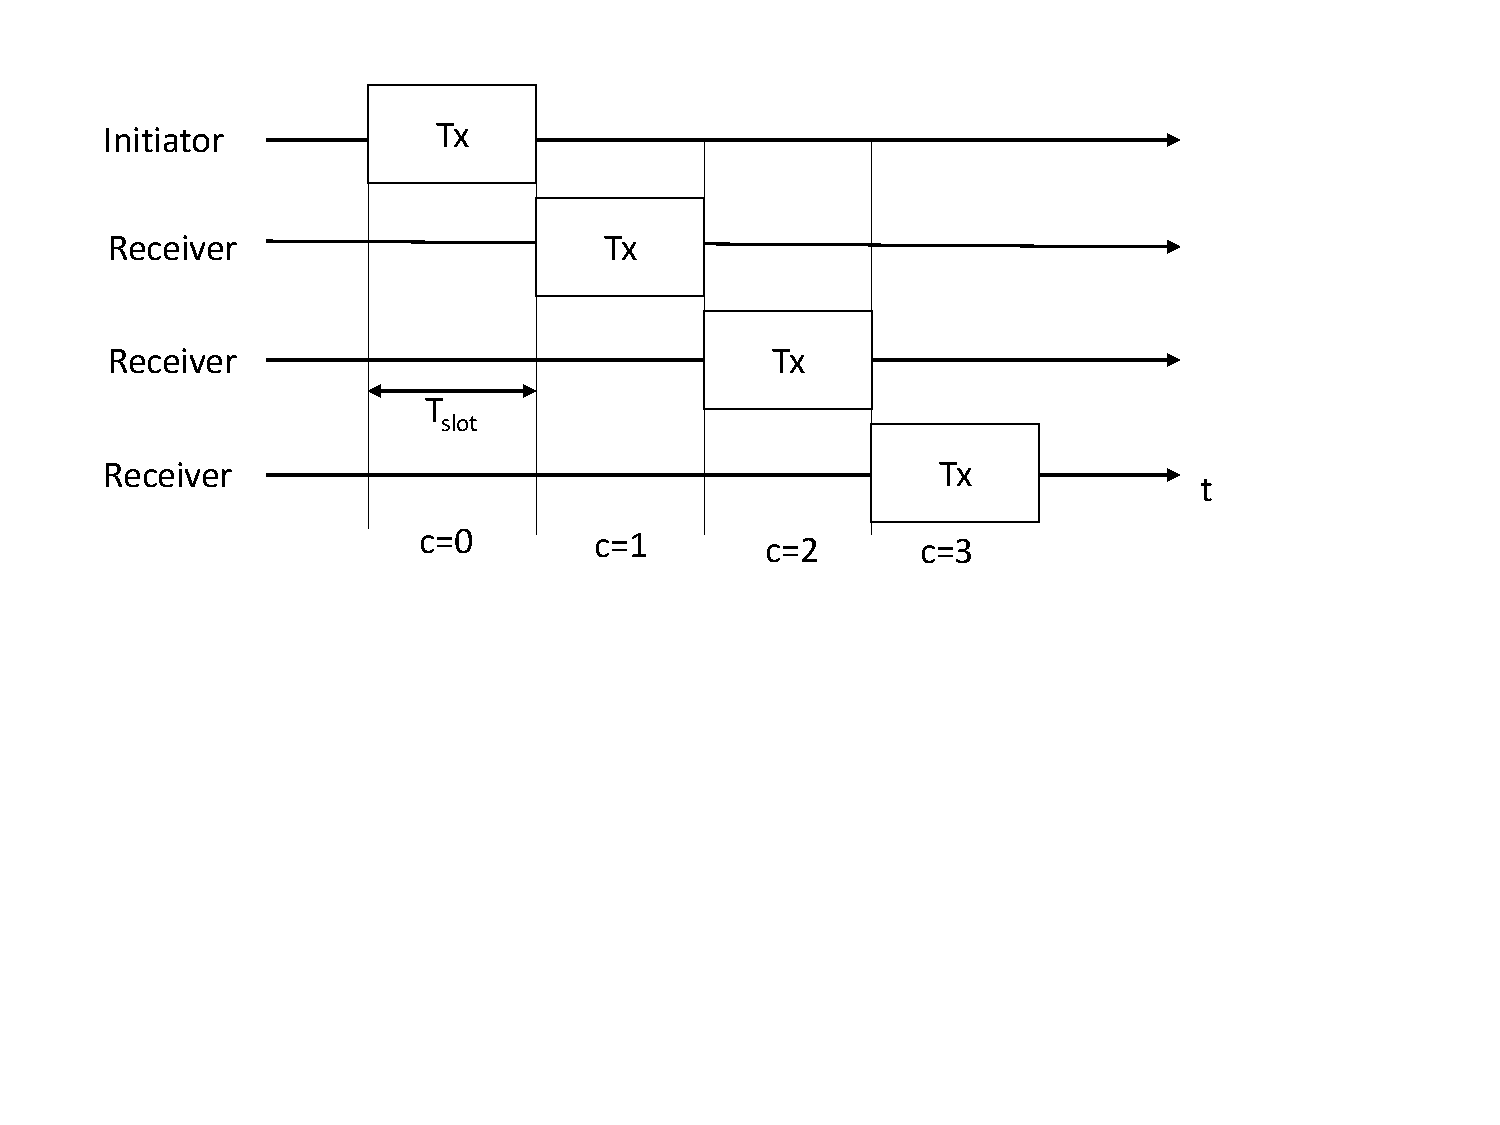
\includegraphics[width=0.9\textwidth]{figures/ts.pdf}
 \vspace{-40mm}
 \caption{Initiatorに対する相対的な時刻同期}
 \label{fig:time}
\end{figure}

同時送信フラッディングでは,従来用いられていた,干渉を避けるため一定時間送信を待つというランダムバックオフが不要なため,受信後即座に転送を行う.そのため理論上では,以下の式\ref{ts}でiホップ目のノードの送信開始時間を表せる.なお,$T_i$はカウンタiのパケットの送信開始時間,$T_{ini}$はInitiatorの基準時間である.
\begin{equation}
\label{ts}
T_i=T_{ini}+c・T_{slot}
\end{equation}

実際にはソフトウェア遅延やハードウェアの違いも考慮した時刻同期が必要で~\cite{Effi}では考慮されているが本研究では簡単のため考慮しない.ここで重要なのは,Initiatorの基準時間とパケット内の中継カウンタから,自分の転送開始時刻がわかること,また自身が保持している時間とパケットの中継カウンタから求まるInitiatorの基準時間を比較すれば,自分が転送に参加すべきかどうかが判断できるという点である.



\section{関連研究}
同時送信フラッディングをセンシング基盤Chocoに実装し,実際に10~70台のセンサノードを用いて,橋梁でのモニタリングに適用した先行研究~\cite{monitoring}においては,「ノードの移動に頑健である」「ネットワークに関する専門的な知識が少なくても構築が容易で利用しやすい」という同時送信フラッディングの有意性が確認されている.

\subsection*{LoRaへの適用}
また,物理層プロトコルLoRaと同時送信フラッディングを組み合わせについて検討し,送信時に意図的に遅延を挟むことでパケットエラー率の抑制を図るオフセットCT法が検討されている~\cite{LoRa}.ここから複数の信号を受信した際,信号間の電力差が小さい場合でも同時送信フラッディングにおいては復調が可能であること,遅延をはさんで送信時間をずらすことでさらに正しく復調できる確率が上がることがわかっている.またホップ数の増加に伴う遅延の拡大を抑制できることも確認されている.オフセットCT法は従来のCT法が苦手とするノードが密集している状況においてPRRを大幅に改善することができる.

\subsection*{トラヒック要求に応じたスケジュール割り当て}
また同時送信フラッディングにおいて,各サービスのトラヒック要求に応じて,スケジュール割り当てを行う試みも行われている~\cite{monitoring}.これにより,トラヒック要求がないときはスリープ,トラヒック要求が多いときは優先的にスロット割り当てを行うことができ,消費電力やデータ収集の点から高効率である.
